

\chapter{Operating Systems}
\label{chap:operating-systems}

In this chapter we provide a survey of existing operating systems and mechanisms for building
mixed-criticality systems. We evaluate
the scheduling and resource sharing policies and mechanisms available, with a focus on temporal isolation,
asymmetric protection, policy freedom, and resource sharing.  
% TODO is asymmetric protection still a thing we want to support?
First we present a number of industry standards, before examining
Linux other open source operating systems, in addition to
commercial offerings, in order to establish current industry standards for temporal isolation.
Finally, we survey existing, relevant operating systems
from systems research, deeply examining techniques that can be leveraged to build mixed-criticality
systems, including isolation and resource sharing techniques.

\section{Standards}

In order to establish standard industry practices, we first present three standards (POSIX, ARINC
653, and AUTOSAR) and examine their mechanisms for temporal isolation and resource sharing.

\subsection{POSIX}

First, we look at the \emph{\gls{POSIX}} standard which underlies many commercial and open-source operating
systems. 
\gls{POSIX} is a family of standards, which includes specifications of \gls{RTOS} interfaces~\citep{Harbour_93} for scheduling and
resource sharing, which
influence much \gls{OS} design.  Scheduling policies specified by \gls{POSIX} are shown in
\Cref{tab:posix-sched}. 

\begin{table}
\centering
\rowcolors{2}{gray!25}{white}
\begin{tabular}{lp{.7\textwidth}}\toprule
    \emph{Policy}  & \emph{Description} \\\midrule
    \schedfifo     & Real-time tasks can run at a minimum of 32 fixed-priorities until they are preempted or yield. \\
    \schedrr       & As per \schedfifo but with an added timeslice. If the timeslice for a thread expires, it is added to the tail of the scheduling queue for its priority.\\
    \schedsporadic & Specifies sporadic servers as described in \Cref{p:sporadic} and can be used
    for temporal isolation. For practical requirements, the POSIX specification of \schedsporadic
    specifies a maximum number of replenishments which is implementation defined. \\\bottomrule
\end{tabular}
\caption{\gls{POSIX} real-time scheduling policies}
\label{tab:posix-sched}
\end{table}

\citet{Faggioli_08} provides an implementation of \schedsporadic, which \citet{Stanovic_BWH_10}
used to show that the POSIX definition of the sporadic server is incorrect and can allow tasks to
exceed their utilisation bound.  The authors provide a modified algorithm for merging and abandoning
replenishments which fixes these problems, of which corrections to the pseudo code were published by
\citet{Danish_LW_11}.  In further work \citet{Stanovic_BW_11} show that while sporadic servers
provide better response times than polling servers under average load, under high load the overhead
of preemptions due to fine-grained replenishments causes worse response times when compared to
polling servers.  Consequently, they evaluate an approach where servers alternate between sporadic
and polling servers depending on load, where the transition involves reducing the maximum number of
replenishments to one and merging available refills.

Resource sharing in the \gls{POSIX} \gls{OS} interface is permitted through mutexes, which can be
used to build higher synchronisation protocols.  \Cref{tab:posix-mutex} shows the specified
protocols. 

\begin{table}
\centering
\rowcolors{2}{gray!25}{white}
\begin{tabular}{lp{.7\textwidth}}\toprule
\emph{Policy} & \emph{Description} \\\midrule
\noprioinherit & Standard mutexes that do not protect against priority inversion. \\
\prioinherit  & Mutexes with \gls{PIP} to prevent priority inversion, recall \Cref{sec:pip}. \\
\prioprotect & Mutexes with \gls{HLP} to prevent priority inversion, recall \Cref{sec:hlp}. \\
\bottomrule
\end{tabular}
\caption{\gls{POSIX} real-time mutex policies for resource sharing.}
\label{tab:posix-mutex}
\end{table}

Although \gls{POSIX} provides \schedsporadic which can be used for temporal isolation (however
flawed), the intention of the policy is to contain aperiodic tasks. 
However, temporal isolation of shared resources is not possible with \gls{POSIX}.
This is because \schedsporadic allows threads to run at a lower priority if 
they have exhausted their sporadic allocation, meaning those threads can still access resources
even when running at lower priorities. In fact, running at lower priorities ensures that threads
contained by sporadic servers can unlock locked resources: however, it also does not bound
locking, or provide ways to pre-empt locked resources.
As a result, \gls{POSIX} is insufficient for
mixed-criticality systems where tasks of different criticalities share resources.  Few \glspl{OS}
implement the full \gls{POSIX} standard, however many incorporate features of it, including Linux.

\subsection{ARINC653}
\label{s:arinc}

\citet{ARINC653} 653 (Avionics Application Standard Software Interface) is a software specification
for avionics which allows for the construction of a limited form of mixed-criticality systems. Under
ARINC 653, software of different criticality levels can share hardware under strict temporal and
spatial partitioning, where CPU, memory and \IO are all partitioned. 

Software of different criticality levels are assigned to separate, non-preemptive partitions, which
are scheduled according to a fixed-time window, in the fashion of a cyclic executive
(recall \cref{s:cyclic-executive}). When a partition switch occurs, all CPU pipeline state and
cache state is flushed to avoid data leakage between partitions~\citep{VanderLeest_10}. Within partitions,
a second-level, preemptive, fixed-priority scheduler is used to dispatch threads, with \gls{FIFO}
ordering for equal priorities. 
At the end of each partition, all CPU pipeline state and cache
state is flushed and a partition switch occurs. Temporal isolation under ARINC is therefore
completely fixed between partitions, and non-existent within partitions. 

The ARINC 653 specification does not consider multiprocessor hardware, although it is possible to
schedule specific partitions on fixed processors. 

The standard does permit resource sharing between partitions: resources are either
exclusive, and accessible to one partition only, or shared between two or more partitions.
Synchronisation mechanisms are specified both inter- and intra-partition. 

Inter-partition sharing between partitions is provided by sending and receiving ports, configured to be either
sampling ports, or queuing ports, depending on the access required~\citep{Kinnan_Wlad_04}.
Importantly, ports have no 
impact on the scheduling order of partitions, all operations must complete in the duration of a
partition's fixed-time window.

Intra-partition synchronisation is via the low-level events and semaphores, or high-level
blackboards and buffers. The latter are both uni-directional 
message passing interfaces, \emph{buffers} provide a statically-sized producer-consumer queue while
\emph{blackboards} provide asynchronous multicast behaviour where multiple tasks can read the latest
message until it is cleared~\citep{Zuepke_BL_15}.
Finally, ARINC 653 specifies a health monitoring system, which can detect deadline misses and run
preconfigured exception handlers.

\subsection{AUTOSAR}

AUTOSAR (AUTomotive Open System ARchitecture) is a set of specifications for developing real-time
software in the automotive domain, which like ARINC653, has a focus on safety. Unlike ARINC, AUTOSAR
does not specifically provide for mixed-criticality.

Software in AUTOSAR is either trusted or untrusted, where trusted indicates it can be run in
privileged mode. This is effectively an all-or-nothing mechanism for spatial isolation, derived
from the fact that much of the hardware AUTOSAR runs on is embedded without an \gls{MMU}, which
would allow for more fine-grained spatial isolation.
In terms of temporal isolation, AUTOSAR provides a mechanism referred to as \emph{timing
protection}, where tasks execution times, resource access durations and inter-arrival times are
specified and monitored, such that exceptions can be raised on temporal
violations~\citep{Zuepke_BL_15}. 

Scheduling in AUTOSAR is partitioned per processor, with a  
fixed-priority, preemptive scheduler per core, with \gls{FIFO} for equal priorities. Unlike ARINC,
AUTOSAR allows for inter-processor synchronisation, facilitated by spinlocks. 

For resource sharing, AUTOSAR specifies synchronisation through \gls{IPCP}, supported by allowing
tasks to raise their priority to the resources' configured priority. Additionally, AUTOSAR supports
nesting of resources. For synchronisation, events are provided, which threads can block on.

\subsection{Summary}

We have surveyed three standards: POSIX, ARINC and AUTOSAR. All mandate the use of fixed-priority schedulers 
and provide protocols and mechanisms for resource sharing. Under POSIX, 
the focus of the resource sharing mechanisms is synchronisation of critical sections for
correctness, not temporal isolation. AUTOSAR provides optional monitoring which can raise an
exception if a task holds a resource for too long, although this requires exact scheduling
details to be provided about the task and resource. ARINC alone provides real temporal isolation for
tasks sharing resources however, the support is limited to fixed, static
partitions with no flexibility.

\section{Existing operating systems}

There is a significant gap between real-time theory, as surveyed in the last chapter, and real-time
practice, which we have partially highlighted in the previous section. Now we survey of existing open-source
and commercial operating systems, which are used in practice, to demonstrate the status quo, and 
the impact of the discussed specifications and standards on their development.

\subsection{Open source}

Many open source \glspl{OS} are used in real-time settings, although generally not in
safety-criticality systems. Regardless, temporal isolation and resource sharing mechanisms remain important to
guarantee the function of the software.

\subsubsection{Linux}

Due to its collaborative development and a massive code base, Linux is not amenable to
certification and cannot be considered an \gls{OS} for high-criticality applications. However, Linux
is frequently used for low-criticality applications with \gls{SRT} demands, and can be used to
provide low-criticality services in a mixed-criticality setting, as long as it is sufficiently
isolated. Additionally, Linux is often used as a platform for conducting real-time systems research. 

% TODO cite completely fair scheduler
Linux has fixed-priority preemptive scheduler which is split into scheduling classes.  Real-time
threads can be scheduled with \gls{POSIX} \schedfifo and \schedsporadic. Best-effort threads are
scheduled with the time-sharing \gls{CFS}, and real-time threads are scheduled either \gls{FIFO} or round-robin, and
are prioritised over the best-effort tasks.  Fixed priority threads in Linux are completely trusted:
apart from a bound on total execution time for real-time threads which guarantees that best-effort
threads are scheduled (referred to as real-time throttling~\citep{Corbet_08}), individual temporal
isolation is not possible.

Linux version 3.14 saw the introduction of an \gls{EDF} scheduling class~\citep{Corbet_09},
which is between the fair and the fixed priority scheduling classes.  The \gls{EDF} implementation
allows threads to be temporally isolated using \gls{CBS}.

Scheduling in Linux promotes the false correlation we see in many systems: real-time tasks are
automatically trusted (unless scheduled with \gls{EDF} and \gls{CBS}) and assumed to be more important---or more
critical---than best-effort tasks.  In reality criticality and real-time strictness are orthogonal.
Linux does not provide any mechanisms for asymmetric protection beyond priority.

On the resource sharing side Linux provides real-time locking via the \gls{POSIX} API as per
\Cref{tab:posix-mutex}, which is unsuitable for mixed-criticality shared resources.

Numerous projects attempt to retrofit more extensive real-time features onto
Linux.  We briefly summarise major and relevant works here. 

One of the original
works~\citep{Yodaiken_Barabanov_97} runs Linux as a fully-preemptable task via virtualisation and
kernel modifications, and runs real-time threads in privileged mode. Interrupts are virtualised and
sent to real-time threads, and only directed to
Linux if required. Consequently, real-time tasks do not have to suffer from long interrupt
latencies, however it also means that devices drivers need to be rewritten from scratch for
real-time. This approach is clearly untenable in a mixed-criticality system, given all real-time
threads are trusted. 

\litmus~\citep{Calandrino_LBDA_06} is an extension of Linux that allows for pluggable real-time
schedulers to be easily developed for testing multiprocessor schedulers which schedule kernel
threads. Real-time schedulers run at a higher priority than best-effort threads, and schedulers can
be dynamically switched at run time. \litmus is not intended for
practical use, but for developing and benchmarking scheduling and resource sharing algorithms.
Implementations of global- and partitioned-, EDF and FP schedulers exist for LITMUS, in addition to
\emph{PFair} schedulers. A \gls{SS} implementation exists, as well as various multicore,
real-time locking protocols.

\linuxrk~\citep{Oikawa_Rajkumar_98} is a resource kernel implementation of Linux with scheduling,
admission control, and enforcement in the kernel. Every resource, memory, CPU time and devices was
time-multiplexed using a recurrence period, processing time and deadline. Reservations in \linuxrk
could be hard, firm of soft, which altered resource scheduling after a resource was exhausted. Hard
reservations were not scheduled again until replenishment, firm would only be scheduled if no other
undepleted reserve or unreserved resource use was scheduled, while soft allowed resource usage to be
scheduled at a background priority. \linuxrk is additionally often used to implement and test other
schedulers, such as \Gls{ZS} scheduling~\citep{deNiz_LR_09}, which was presented in
\cref{s:zero-slack-scheduling}.
 
Whilst Linux implementations are suitable for implementing algorithms, being used as test-beds and
even being deployed for non-critical \gls{SRT} applications, ultimately Linux is not a suitable
\gls{RTOS} for running safety-critical \gls{HRT} applications. The large amount of source code
results in a colossal trusted computing base, where it is impossible to guarantee correctness through
formal verification or timeliness through {\gls{WCET}} analysis.  Major reasons for adapting Linux
to real-time are the existing applications and wide array of device and platform support. For
mixed-criticality systems these advantages can be leveraged by running Linux as a virtualised, guest \gls{OS} to run \gls{SRT}
and best-effort applications.

\subsubsection{RTEMS}

\citet{RTEMS:URL} is an open-source \gls{RTOS} that operates with or without memory protection,
although in either case it is statically configured.  Although it is an open source project, RTEMS
is used widely in industry and research.  The main scheduling policy is \gls{FPRM}, however
\gls{EDF} is also available with temporal isolation an option using \gls{CBS}.  No temporal
isolation mechanisms are present for fixed-priority scheduling.  RTEMS provides semaphores with
\gls{PIP} or \gls{HLP} for resource sharing, as well as higher level primitives for these. RTEMS
does not provide mechanisms for shared resources, as target threads are trusted to complete critical
sections within a determined \gls{WCET}, and provides no mechanism for isolation through shared
resources.

\subsubsection{FreeRTOS}

\citet{FreeRTOS:URL} is another open-source \gls{RTOS}, however it only supports systems with \glspl{MPU}, not
\glspl{MMU}. The scheduler is preemptive \gls{FP} and \gls{PIP} is provided to avoid priority inversion.
%FreeRTOS can be configured to be tickless or not.


\subsection{Commercial RTOSes}
%TODO add details on resource sharing to this section
Several widely deployed \glspl{RTOS} are used commercially, the majority providing support for part or
all of \gls{POSIX}.  

\subsubsection{QNX Neutrino}

\citet{QNX_10} was one of the first commercial microkernels, widely used in the transport industry.
QNX is a separation based, first-generation microkernel that provides
\gls{FP} scheduling and resource sharing with POSIX semantics.  QNX satisfies many industry
certification standards, although these in practice do not require {\gls{WCET}} analysis or formal
verification of correctness. 

\subsubsection{VxWorks}

VxWorks~\citep{VxWorks_08} is a monolithic \gls{RTOS} deployed most notably in aircraft
and spacecraft.  It supports \gls{FP} scheduling with a native POSIX-compliant scheduler, and
implements ARINC 653.  VxWorks
also has a pluggable scheduler framework, allowing developers to implement their own, in-kernel
scheduler.

\subsubsection{PikeOS}

PikeOS~\citep{PikeOS:URL} is a second-generation microkernel which implements ARINC 653~\citep{ARINC653} 
and runs RTOSes as paravirtualised guests in different partitions. Partitions are scheduled
statically in a cyclic fashion, and each partition has its own scheduling structure supporting 256
priorities.
An alternative design has been implemented for PikeOS~\citep{Vanga_BTB_17}, where reservations are
used to schedule low-latency, low-criticality tasks.
This is achieved by using ``\gls{EDF} within fixed priorities''~\citep{Harbour_Palencia_03}, which
schedules using EDF at specific priority bands, combined with a pluggable interface for using a
reservation algorithm (\eg \gls{CBS}, \gls{SS}, \gls{DS}) to temporally contain threads. In order to achieve low-latency, these tasks are run
in the special partition of PikeOS, known as the system partition, which is scheduled at the same
time as the currently active partition and provides essential system services. However, these tasks
are intended to run without sharing resources or interfering with high-criticality tasks, which run
in their own partitions.

\subsubsection{Deos}

\citet{Deos:URL} is another RTOS which provides fixed-priority scheduling, with the addition of slack
scheduling, where threads can register to receive slack and are scheduled according to their
priority when there is slack in the system. Like PikeOS, Deos also implements ARINC 653 and a
defined subset of POSIX.

\subsection{Summary}

There are many other \gls{RTOS}es used commercially, but the general pattern is POSIX-compliant, 
\gls{FP} scheduling and resource sharing.
This brief survey shows that \gls{FP} scheduling is dominant in industry due to its predictable
behaviour on overload, specification in the
POSIX standard, and compatibility with existing, priority-based, best-effort systems. 
If \gls{EDF} is incorporated, it is provided at priority bands in the fixed-priority system.
Without a principled way to treat time as a first-class resource, the reliance on fixed-priority
conflates the importance of a task and its scheduling priority, often based on rate, resulting in 
low utilisation in these systems.

\begin{table}[h]
\centering
\rowcolors{2}{}{gray!25}
\begin{tabular}{lll}\toprule
  \emph{OS} & \emph{Scheduler}  & \emph{Temporal Isolation} \\\midrule
Linux       & \gls{FP} + \gls{EDF} & \gls{CBS} \\
RTEMS       & \gls{FP} + \gls{EDF} & \gls{CBS} \\
FreeRTOS    & \gls{FP}             & \no       \\
QNX         & \gls{FP}             & ARINC 653, \gls{SS} \\ 
VxWorks     & \gls{FP}             & ARINC 653   \\
PikeOS      & \gls{FP}             & ARINC 653    \\
Deos    & \gls{FP}             & ARINC 653\\
\bottomrule
\end{tabular}
\label{t:os-summary}
\caption{Summary of scheduling and temporal isolation mechanisms in surveyed open source and
commercial \glspl{OS}.}
\end{table}

Although temporal isolation is sometimes provided with the possibility of bounded bandwidth via
\gls{CBS} and or \gls{SS}, support for temporal isolation in 
shared resources is non-existent beyond the strict partitioning of ARINC 653.
Although many of
these \glspl{RTOS} are deployed in safety critical systems, their support for mixed-criticality
applications is limited to the ARINC653 approach discussed in \cref{s:arinc}. Clearly, more flexible 
mechanisms for temporal isolation and resource sharing are required.

\section{Isolation mechanisms}

We now look to systems research and explore mechanisms for temporal isolation and resource sharing
in research operating systems, exploring their history and the state of the art. First, we briefly
introduce each operating system that is surveyed, before exploring in detail specific mechanisms
that can be used to support mixed-criticality systems. We investigate how different \glspl{OS}
address resource kernel concepts required to treat time as a first class resource; scheduling,
accounting, enforcement, admission. Additionally, we look at how prioritisation, charging and
enforcement are achieved, if at all, to achieve temporal isolation across shared resources.

The majority of kernels surveyed here are microkernels, as introduced in
\cref{sec:background-operating-systems} and are as follows: 

\begin{itemize}
    \item Real-time Mach~\citep{Mercer_RZ_94, Mercer_ST_93}, a first-generation microkernel.
    \item The \gls{DROPS}~\citep{Haertig_BBHHMRSW_98}, a second
        generation, L4 microkernel.
    \item EROS~\citep{Shapiro_SF_99}, the first third-generation microkernel.
    \item Fiasco~\citep{Hohmuth_02} is a second-generation L4 microkernel, with fixed-priority scheduling.
    \item Tiptoe~\citep{Craciunas_KPRS_09} is a now-defunct research microkernel that also aims at
temporal isolation between user-level processes and the operating system.
    \item NOVA~\citep{Steinberg_Kauer_10} a third-generation microkernel and hypervisor.
    \item \composite~\citep{Parmer:phd} is a component-based \gls{OS} with similar with goals to a microkernel,
however with a more dominant focus on support for fine-grained components, and massive scalability.
    \item \citet{FiascoOC:URL}, a third-generation iteration of Fiasco, both microkernel and
        hypervisor.
    \item Barrelfish~\citep{Peter_SBBIHR_10} is a capability-based multi-kernel \gls{OS}, where a separate kernel runs on each processing core and kernels themselves share no memory and are essentially \emph{\gls{CPU}-drivers}.
    \item Quest-V~\citep{Danish_LW_11} is a separation kernel / hypervisor.
    \item \selfour~\citep{Klein_AEMSKH_14}, a third-generation microkernel with
        hypervisor support and a proof of functional correctness. We present \selfour 
        and its mechanisms in more detail in \cref{chap:sel4}.
\end{itemize}


\subsection{Scheduling}

As in commercial and open source \glspl{OS}, fixed-priority scheduling dominates in research, with
only Tiptoe and Barrelfish providing \gls{EDF} schedulers, although \minix has been adapted for 
real-time~\citep{Mancina_LFHGT_09}, by allowing the kernel's best-effort scheduling to be
set to \gls{EDF} on a per-process basis.   

\composite stands out, as it does not provide a scheduler or blocking semantics in the kernel at all,
requiring user-level
components to make scheduling decisions. \hires~\citep{Parmer_West_11} is a hierarchical scheduling framework built on top
of \composite. 
 \hires delivers timer interrupts to a root, user-level scheduling component, which are then forwarded
through the hierarchy to child schedulers.  Consequently, scheduling overhead increases as the
hierarchy deepens.  Child schedulers with adequate permissions use a dedicated system call to tell
the kernel to switch threads, while the kernel itself does not provide blocking semantics, which are also
provided by user-level schedulers.  This design offers total scheduling policy freedom, as
user-level scheduling components can implement all the goals of a resource kernel according to
their own policy.

\subsection{Timeslices and meters}
\label{s:timeslices-and-meters}

Meters were one of the first mechanisms used to treat time as a resource, originating 
in KeyKOS ~\citep{Bomberger_FFHLS_92}. A \emph{meter} represented a
defined length of processing time, and threads required meters to execute. Once a meter was
depleted a higher authority was required to replenish it, requiring another thread to run.

L4 kernels~\citep{Elphinstone_Heiser_13} extended this concept with timeslices, 
which like meters are consumed as threads execute, but no
authority is invoked to replenish the meter: the timeslice simply represents an amount of time 
that a thread could execute at a priority before preemption. 
On preemption, the thread placed at the end of
the \gls{FIFO} scheduling queue for the appropriate priority, with a refilled timeslice, in a
round-robin fashion. 

Meters and timeslices provide a unit of time, but do not restrict \emph{when} that time must be consumed
by. Although simpler, timeslices have insufficient policy freedom in that they are recharged immediately,
providing no mechanism for an upper bound on execution. Although meters allowed a user-level policy 
to define replenishment, this proved expensive on the systems and hardware at the time, as every
preemption resulted in a switch to a user-level scheduler and back. Neither concept provides
anything resembling a bandwidth or share of a CPU, and only threads at the highest priority level
have any semblance of temporal isolation as they cannot be preempted by other threads, sharing their
time only with threads at the same priority.

As a result, in a system where time is treated as a first-class resource,
the timeslice/meter is not an appropriate, policy-free mechanism alone for building mixed-criticality
systems with temporal isolation guarantees.

\subsection{Reservations}
% TODO finish unifying

Many research \glspl{OS} have provided mechanisms for processor reservations, a concept with roots
in resource kernels, as introduced in \label{sec:resource-kernels}. Like meters and timeslices,
reservations are consumed when threads execute upon them, however, they represent a bandwidth or
share of a processor, and provide a mechanism for temporal isolation.

Reservation schemes differ in the algorithm used to ensure the specified bandwidth was not
exceeded: Mach and EROS used \gls{DS}, Tiptoe \gls{CBS}, while Barrelfish provides \gls{RBED}. 
\Glspl{SS} are provided by Quest-V~\citep{Li_WCM_14}, which address the back-to-back
problem of \gls{DS} however require a more complex implementation.
Quest-V~\citep{Danish_LW_11} provides reservations through \gls{SS}, however \IO and normal processes
are distinguished statically: \IO processes use polling servers and normal processes use sporadic
servers. 

All the research OSes that implement reservations have an admission
test in the kernel which is run on new reservations, and checks that the set of reservations are
schedulable. Although the testing is done dynamically, providing the admission test in the kernel makes the scheduler used, and the
schedulability test, an inflexible policy mandated by the kernel. 

Enforcement policy, which determines what occurs when a reserve is exhausted,
varies between two extremes: either threads cannot be scheduled until the reservation is
replenished, or it is scheduled in slack time. 
\gls{CBS} approaches enforce an upper bound on execution, not permitting threads to run until 
replenishment. Real-time Mach, with EROS to follow, allowed threads with exhausted reservations to
run in a second-level, time-sharing scheduler. For RBED-based approaches, enforcement is coded into
the classification of the task: rate-based tasks are not scheduled until replenishment, but
best-effort and \gls{SRT} tasks can run in slack time. 
\gls{DROPS} allowed processes to reserve a 
higher priority for a certain amount of cycles, before returning to a lower priority, essentially
running expired reservations in slack time. 

The importance or reservations also varies. In the case of RBED, the highest criticality threads
are trusted, and their execution is not monitored at all, while threads with reservations are
considered second tier and best-effort threads the least important. This allows for a strict form 
of asymmetric protection where \gls{HRT} threads can temporally effect \gls{SRT} threads and
best-effort threads, but not vice-versa. The Mach approach, on the other hand, only guarantees time
to threads with reservations, which are scheduled ahead of any threads in the time-sharing
scheduler. We consider both models to be policy, as is the original resource kernel concept where
all threads must have a reservation in order to execute at all.  

Some implementations allow for multiple threads to run on one reservation, which effectively creates
a hierarchical scheduler, but allows for convenient temporal isolation of a set of tasks. In
Quest-V, reservations are actually bound to virtual processors, not threads scheduled by that
processor. 

Reservations are a mechanism that can be used to provide isolation, however, all the kernels
surveyed combine this mechanism with a good deal of policy for enforcement, how important
reservations are, and admission. To build mixed-criticality systems, we
need high-performance mechanisms for temporal isolation that are decoupled from policy.

\subsection{Timeslice donation}

Reservations alone can be used to provide temporal isolation, however are insufficient without
further mechanisms for resource sharing. Recall from \cref{p:resource-kernel-resource-sharing} that
prioritisation (the priority threads use when accessing resources), charging (which reservation to
charge during resource access) and enforcement (what action to take when a reservation expires while
accessing a resource) are key to avoiding priority inversion in a resource kernel.

We first examine mechanisms for charging in the context of microkernels.
Recall from \cref{s:background-ipc} that in a microkernel, \gls{OS} services are implemented at
user-level where clients use \gls{IPC} to communicate with servers, in an \gls{RPC}-like fashion, as
illustrated in \cref{f:os-ipc}. These servers logically map to shared resources, where clients are
the threads accessing those resources.

\begin{figure}
    \centering
    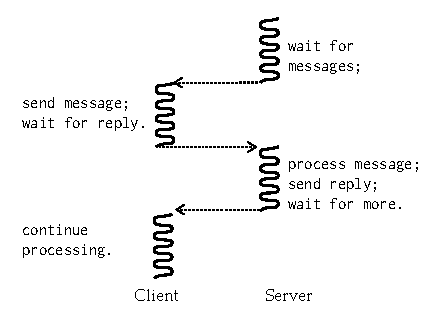
\includegraphics[width=0.8\textwidth]{ipc-port}
    \caption{Thread execution during IPC between client and server}
    \label{f:os-ipc}
\end{figure}

Early implementations of IPC had clients send messages directly to servers by referencing the
thread ID. Later IPC message \emph{ports} were introduced to provide isolation; clients send
messages and wait for replies on ports, and servers receive messages on ports and reply to the
client's message on that port, removing the need for threads to know details about each other. 
Servers effectively provide resources shared with multiple clients, via IPC through ports. 

The heavy optimisation of second- and third-generation microkernels resulted in \emph{timeslice
donation}, and optimisation which avoided the scheduler~\citep{Heiser_Elphinstone_16}. 
Timeslice donation works as follows: the client calls the server, if the server is higher or equal
priority it is switched to directly without invoking the scheduler at all, effectively a yield.
The intuition is that in
a fast IPC system, the request should be finished before the timeslice expires. In reality, longer
requests do occur, so while the clients timeslice is used for the start of the request, the servers
timeslice is used beyond that. This results in no
proper accounting of the server's execution, and no temporal isolation.

Other kernels, like Barrelfish, allowed the sender to set a flag on a message specifying if
timeslice donation should occur. However, this approach still suffers the problem of undisciplined 
charging, rendering timeslice donation an inappropriate mechanism for temporal isolation over
shared resources.

\subsubsection{Scheduling contexts}
\label{s:sc-intro}

The mechanism of scheduling contexts is a more principled extension of timeslice donation.
Thread structures in the majority of kernels contain the execution context (registers) and scheduling
information, such as priority and accounting information, in a single structure known as a \gls{TCB}.
Other kernels, including real-time Mach, NOVA, and \fiascooc, divide the TCB into an execution context and
\emph{scheduling context} in order to allow the scheduling context to
transfer between threads over \gls{IPC} for accounting and/or priority inheritance purposes, and for
performance~\citep{Steinberg_Kauer_10}.

The contents of a scheduling context vary per implementation.
Real-time Mach's scheduling contexts contained parameters for the deferrable
server, while NOVA's contained a timeslice. In \fiascooc, scheduling contexts contain a
replenishment rule, and a budget. All three implementations include a priority in the
scheduling context. 

\emph{Scheduling context donation} refers to a scheduling context transferring between threads over
\gls{IPC}, and is implemented in both Real-time Mach and NOVA, although the implementations are
quite different. We look at both in terms of prioritisation, charging, and enforcement. 

In Real-time Mach, scheduling donation would always occur and the scheduling context of the client
always charged. In terms of prioritisation, a flag on the message port
indicated if the server should run at the priority of the scheduling context, or a statically set
priority. A further flag indicated if \gls{PIP} should be implemented, where the server's priority
would be increased to the priority of scheduling contexts from further pending requests~\citep{Kitayama_NT_93}. Although this approach provided a fair amount of policy freedom, it introduces performance costs on the 
critical \gls{IPC} path, on a kernel already notorious for its poor \gls{IPC}
performance~\citep{Hartig_HLSW_97}. 
The enforcement policy of Real-time Mach derived directly from its two-level scheduler, and if a
scheduling context expired the server would run in the second-level time-sharing scheduler, blocking
any pending requests.

NOVA~\citep{Steinberg_BK_10} also provided scheduling contexts with donation over \gls{IPC},
although the prioritisation policy was strictly \gls{PIP}, which has high preemption overhead, 
as described in \cref{sec:pip}, and conflicts with the
policy-freedom goal of a microkernel. 
Enforcement and charging
in NOVA are both provided through the mechanism of helping:  a form of
bandwidth inheritance, where pending clients not only boost the priority of the server, but the
server can charge the current clients request to the pending client in order to finish the initial request. 

In both implementations of scheduling context donation, the charging mechanism becomes policy: the
scheduling context of the client is always charged. Although Mach provided a mechanism to allow for
system-specific prioritisation, this came at a considerable IPC cost. Finally, both provide
different enforcement mechanisms but both are hard-coded policy which rely on either charging the
next client, or running in slack. While scheduling contexts are a good mechanism for
passing reservations across \gls{IPC}, and thereby implementing temporal isolation over shared
resources, the state of the art is insufficient.


\subsection{Capabilities to time}
\label{s:os-capabilities}

Recall from \cref{s:b-capabilities} that capabilities~\citep{Dennis_VanHorn_66} are an established mechanism for
fine-grained access control to system resources.
Third-generation microkernels use capabilities for principled access to system resources, including 
KeyKOS, EROS, \fiascooc, NOVA, \selfour, \composite and Barrelfish. Of those, only KeyKOS, EROS and
\composite apply the capability system to processing time, we explore these systems after
differentiating temporal and spatial capabilities. 

The major challenge of applying capabilities to time is the fact that time cannot be treated
as fungible. This is very different to spatial resources like memory, which is rendered fungible by the
flexibility of virtual memory systems: it where a page of memory is, as long as it has the correct
contents. One window of time is not replaceable for another window, even in the case of a
best-effort task: a minor change in schedule can force a deadline miss somewhere else.
Consider real estate: like time, it is (arbitrarily) divisible but not fungible: If
a block is too small to build a house, then having a second,
disconnected block of the same size is of no help (unlike spatial resources in a kernel, which can
be mapped side-by-side). The implication is
that capabilities for time have a different flavour from those for
spatial resources---they cannot support hierarchical delegation
without loss, and cannot be recursively virtualised. While delegation is an
attractive property of spatial capabilities,
this delegation is not their defining characteristic, which is actually
\emph{prima facie evidence of access}; in the case of time
capabilities, the access is to processor time.
Previous implementations all have caveats and limitations, which we now detail.


KeyKOS provided capabilities to \emph{meters}, which granted the holder
the right to execute for the unit of time held by the meter, however as established in 
\cref{s:timeslices-and-meters}, meters are not a suitable mechanism for temporal isolation.

EROS~\citep{Shapiro_SF_99} combined processor capacity reserves with capabilities rather than the
meters of KeyKOS. Additionally, 
However, processor capacity reserves were \emph{optional}: a two level scheduler first
scheduled the reserves with available capacity, then threads without reserves,
or with exhausted reserves, were scheduled.
Like any hierarchical scheduling model, this enforces a policy that
reduces flexibility.
Furthermore, hierarchical delegation has the significant disadvantage
of algorithmic utilisation loss~\citep{Lackorzynski_WVH_12}; this is a
direct result of the unfungible nature of time.

\composite recently introduced temporal capabilities~\citep{Gadepalli_GBKP_17} reminiscent of
the meters of KeyKOS in that they represent a scalar unit of time. 
Unlike KeyKOS, temporal capabilities integrate with user-level scheduling, decoupling access control
from scheduling. An initial capability \emph{Chronos} provides authority to all time, and is used to
provide an initial allocation of time and for further replenishment. 
The kernel up calls user-level schedulers 
which must then provide not only a thread to run, but a temporal capability to drain time from.
On expiry, the user-level scheduler is also
invoked, however this is a rare occasion as a well-built scheduler will ensure threads have
sufficient capabilities on each scheduling decision.
 A notion of \emph{time quality} supports delegation across
hierarchically-scheduled subsystems without explicitly mapping all
local priorities onto a single, global priority space, although for performance reasons, the number
of supported delegations is statically limited.
Additionally, time capabilities cannot be revoked unless empty. 
\composite's mechanism of temporal capabilities is the most promising, and decoupling access
control from scheduling is surely key to providing mechanisms for temporal isolation without 
heavily restricting policy freedom. However, the static limit on delegations and lack of revoke
makes the design incomplete for a production system, revoke is generally the hardest part to
implement in a capability system. 

\section{Summary}
% TODO rewrite to reflect update
In this chapter we have reviewed standards and specifications for real-time operation systems,
commercial and open-source real-time operation systems, and finally, surveyed the state-of-the-art
research into mechanisms for temporal isolation, resource sharing, and access control to processing
time.

While real-time literature is divided between which real-time scheduling algorithm should be
deployed as the core of real-time systems (\gls{EDF} or \gls{FP}), no such divide exists in industry
where the all \glspl{OS} provide \gls{FP}. 
Except in a pure research sense, kernels that provide
\gls{EDF} do so in addition to \gls{FP}.  Resource reservations and \gls{EDF} are more common in
research OSes, whilst commercial and open source products are heavily influenced by ARINC 653 and
provide static partitioning. 
 
As we have seen, many existing systems conflate criticality and time sensitivity 
in a single value: priority. A further assumption is that high criticality, time-sensitive tasks are
always trusted, one the falls apart in the mixed criticality context. 

The \emph{criticality} of a component reflects its importance to the
overall system mission.
Criticality may reflect the impact of failure~\citep{ARINC653} or the
utility of a function. An MCS should degrade gracefully, with
components of lower criticality (which we will for simplicity refer to
as \crit{low} components) suffering degradation before higher
criticality (\crit{high}) components.

\emph{Time sensitivity} refers to how important it is to a thread to
get access to the processor at a particular time. For best-effort activities, time is
fungible, in that only the amount of time allocated is of
relevance. In contrast, for a hard real-time component, time is
largely unfungible, in that the allocation has no value if it occurs after
the deadline; soft real-time components are in between.

Finally, \emph{trust} refers to the degree of reliance in the correct
behaviour of a component. Untrusted components may fail completely
without affecting the core system mission, while a component which
must be assumed to operate correctly for achieving the overall mission
is trusted. A component is \emph{trustworthy} if it has undergone a process
that establishes that it can be trusted, the degree of trustworthiness
being a reflection of the rigour of this process (testing,
certification, formal verification)~\citep{Verissimo_NC_03}.

In practice, criticality and trust are closely aligned, as the most
critical parts should be the most trustworthy.
However, criticality must be decoupled from time sensitivity in MCS.
Referring back to the
example in the introduction, interrupts from networks or buses have
high time sensitivity, but low criticality (i.e.\ deadline misses are
tolerable), while the opposite is true for the flight control component.
Similarly, threads (other than the most critical ones which should
have undergone extensive assurance) cannot be
trusted to honour their declared WCET.

Our claim is that how these attributes are conflated is
policy that is specific to a system.
We need a mechanism that allows  enforcing time limits, and thus
isolate the timeliness of critical threads from those of untrusted,
less critical ones.
Reservation-based kernels often allow for a form of over-committing where
best-effort threads are run in the slack-time left by unused reservations or unreserved CPU.
However, this also aligns criticality and time-sensitivity, and
enforces a two-level scheduling model.

If trustworthiness and real-time sensitivity are not conflated, many assumptions about real-time
scheduling fail.
Much real-time analysis rely on threads having a known \gls{WCET}, which implies that those threads
are predictable, which implies trust.
If a real-time thread is not expected to behave correctly, one cannot
assume it will surrender access to the processor voluntarily.
Consequently, the \gls{PIP}/\gls{BWI} based scheduling-context donation mechanisms seen in this chapter are
insufficient, forcing not only a protocol which causes extensive preemption overhead, but 
requiring shared servers to have known, bounded execution time on all requests.

In the next chapter we present a model for mixed-criticality scheduling that is suitable for high
assurance systems such as \selfour. 
